\documentclass[letterpaper,10pt]{amsart}

\usepackage[pdftex]{graphicx}
\usepackage{moreverb}
\usepackage{amsmath}
\usepackage{amsthm}
\usepackage{fullpage}
\usepackage{amssymb}
\usepackage{tikz}
\usepackage{dsfont}
\usepackage{hyperref}
\usepackage[all]{xy}
\usepackage{bbm}
\usepackage{mathtools}
\usepackage[margin=0.5in]{geometry}
\usepackage{enumerate}
\usepackage{multirow}
\usepackage{cancel}


\newcommand{\sumin}{\sum_{i=1}^n}
\newcommand{\sumjn}{\sum_{j=1}^n}
\newcommand{\sumiN}{\sum_{i=1}^N}
\newcommand{\sumjN}{\sum_{j=1}^N}
\newcommand{\sumim}{\sum_{i=1}^m}
\newcommand{\sumjm}{\sum_{j=1}^m}
\newcommand{\prodin}{\prod_{i=1}^n}
\newcommand{\rmd}{\mathrm{d}}
\newcommand{\dx}{\,\mathrm{d}x}
\newcommand{\dy}{\,\mathrm{d}y}
\newcommand{\dt}{\,\mathrm{d}t}
\newcommand{\dz}{\,\mathrm{d}z}
\newcommand{\dmu}{\,\mathrm{d}\mu}
\newcommand{\dnu}{\,\mathrm{d}\nu}
\newcommand{\dP}{\,\mathrm{d}\mathbb{P}}
\newcommand{\fa}{\; \forall \;}


%distributions and functions
\newcommand{\E}[1]{\mathbb{E}\!\left[#1\right]}
\newcommand{\Esub}[2]{\mathbb{E}_{#1}\left[#2\right]}
\newcommand{\p}[1]{\mathbb{P}\!\left(#1\right)}
\newcommand{\psub}[2]{\mathbb{P}_{#1}\left(#2\right)}
\newcommand{\tr}{\operatorname{tr}}
\newcommand{\Var}{\operatorname{Var}}
\newcommand{\Cov}{\operatorname{Cov}}
\newcommand{\Corr}{\operatorname{Corr}}
\newcommand{\argmax}{\operatorname*{arg \, max}}
\newcommand{\argmin}{\operatorname*{arg \, min}}
\newcommand{\Beta}{\textnormal{Beta}}
\newcommand{\Bin}{\textnormal{Bin}}
\newcommand{\logit}{\operatorname{logit}}
\newcommand{\Gammadist}{\textnormal{Gamma}}
\newcommand{\Geom}{\textnormal{Geom}}
\newcommand{\Expo}{\textnormal{Expo}}
\newcommand{\Pois}{\textnormal{Pois}}
\newcommand{\Unif}{\textnormal{Uniform}}
\newcommand{\Bern}{\textnormal{Bern}}
\newcommand{\sgn}{\operatorname{sgn}}
\newcommand{\Mult}{\textnormal{Mult}}
\newcommand{\MVN}{\textnormal{MVN}}


%special letters
\newcommand{\sA}{\mathcal{A}}
\newcommand{\sB}{\mathfrak{B}}
\newcommand{\sC}{\mathcal{C}}
\newcommand{\sD}{\mathcal{D}}
\newcommand{\sF}{\mathcal{F}}
\newcommand{\sG}{\mathcal{G}}
\newcommand{\sH}{\mathcal{H}}
\newcommand{\sI}{\mathcal{I}}
\newcommand{\sL}{\mathcal{L}}
\newcommand{\sN}{\mathcal{N}}
\newcommand{\sP}{\mathcal{P}}
\newcommand{\sQ}{\mathbb{Q}}
\newcommand{\sR}{\mathbb{R}}
\newcommand{\sS}{\mathcal{S}}
\newcommand{\sT}{\mathcal{T}}
\newcommand{\sX}{\mathcal{X}}
\newcommand{\indep}{\perp\!\!\!\perp}
\newcommand{\io}{\text{ i.o.}}

\newtheorem*{prop}{Prop}
\newtheorem{theorem}{Theorem}
\newtheorem*{claim}{Claim}
\newtheorem*{corollary}{Corollary}
\newtheorem{defn}{Definition}
\newtheorem{ex}{Example}
\newtheorem*{lemma}{Lemma}
\newtheorem*{exercise}{Exercise}

\newenvironment{verbatimcode}{\bigskip \scriptsize \verbatim}{\endverbatim \normalsize \bigskip}
\allowdisplaybreaks

\begin{document}

\title{STAT 221 - Assignment 5}
\author{Greg Tam, Student ID: 70908239}
\date{}
\maketitle


\begin{enumerate}[{1}.1]
\item 
The data are written out as a list, but entries in the list may belong to different categories. We need to group them by category, then we can plot them. 

\begin{verbatimcode}
dat = read.csv("1router_allcount.dat")
attach(dat)

nme
levels(nme)
x.corp=c("corp->corp","fddi->corp","local->corp","switch->corp")
x.fddi=c("corp->fddi","fddi->fddi","local->fddi","switch->fddi")
x.local=c("corp->local","fddi->local","local->local","switch->local")
x.switch=c("corp->switch","fddi->switch","local->switch","switch->switch")
x.src=c("src corp", "src fddi", "src local", "src switch")


x.corp=c("corp->corp","corp->fddi","corp->local","corp->switch")
x.fddi=c("fddi->corp","fddi->fddi","fddi->local","fddi->switch")
x.local=c("local->corp","local->fddi","local->local","local->switch")
x.switch=c("switch->corp","switch->fddi","switch->local","switch->switch")
x.src=c("src corp", "src fddi", "src local", "src switch")

x.corp=c("src corp", "dst corp")
x.fddi=c("src fddi", "dst fddi")
x.local=c("src local", "dst local")
x.switch=c("src switch", "dst switch")


corp.index = which(nme %in% x.corp)
fddi.index = which(nme %in% x.fddi)
local.index = which(nme %in% x.local)
switch.index = which(nme %in% x.switch)

par(mfrow=c(4,1),oma=c(1.5,1.5,1.5,1.5))
par(mar=c(3,3,1,0))
corp.index = t(sapply(1:2,function(i) which(nme %in% x.corp[i])))
corp.val = matrix(,nrow=nrow(corp.index),ncol=ncol(corp.index))
corp.val[1,] = value[corp.index[1,]]
corp.val[2,] = value[corp.index[2,]]
plot(corp.index[1,],corp.val[1,],type='l',ylim=range(min(corp.val),max(corp.val)),main="corp")
lines(corp.index[2,],corp.val[2,])

local.index = t(sapply(1:2,function(i) which(nme %in% x.local[i])))
local.val = matrix(,nrow=nrow(local.index),ncol=ncol(local.index))
local.val[1,] = value[local.index[1,]]
local.val[2,] = value[local.index[2,]]
plot(local.index[1,],local.val[1,],type='l',ylim=range(min(local.val),max(local.val)),main="local")
lines(local.index[2,],local.val[2,])

switch.index = t(sapply(1:2,function(i) which(nme %in% x.switch[i])))
switch.val = matrix(,nrow=nrow(switch.index),ncol=ncol(switch.index))
switch.val[1,] = value[switch.index[1,]]
switch.val[2,] = value[switch.index[2,]]
plot(switch.index[1,],switch.val[1,],type='l',ylim=range(min(switch.val),max(switch.val)),main="switch")
lines(switch.index[2,],switch.val[2,])

fddi.index = t(sapply(1:2,function(i) which(nme %in% x.fddi[i])))
fddi.val = matrix(,nrow=nrow(fddi.index),ncol=ncol(fddi.index))
fddi.val[1,] = value[fddi.index[1,]]
fddi.val[2,] = value[fddi.index[2,]]
plot(fddi.index[1,],fddi.val[1,],type='l',ylim=range(min(fddi.val),max(fddi.val)),main="fddi")
lines(fddi.index[2,],fddi.val[2,])

mtext("Origin Destination",outer=TRUE)
mtext("Bytes/sec",outer=TRUE,side=2)
mtext("Hour of Day",outer=TRUE,side=1)
\end{verbatimcode}
\begin{center}
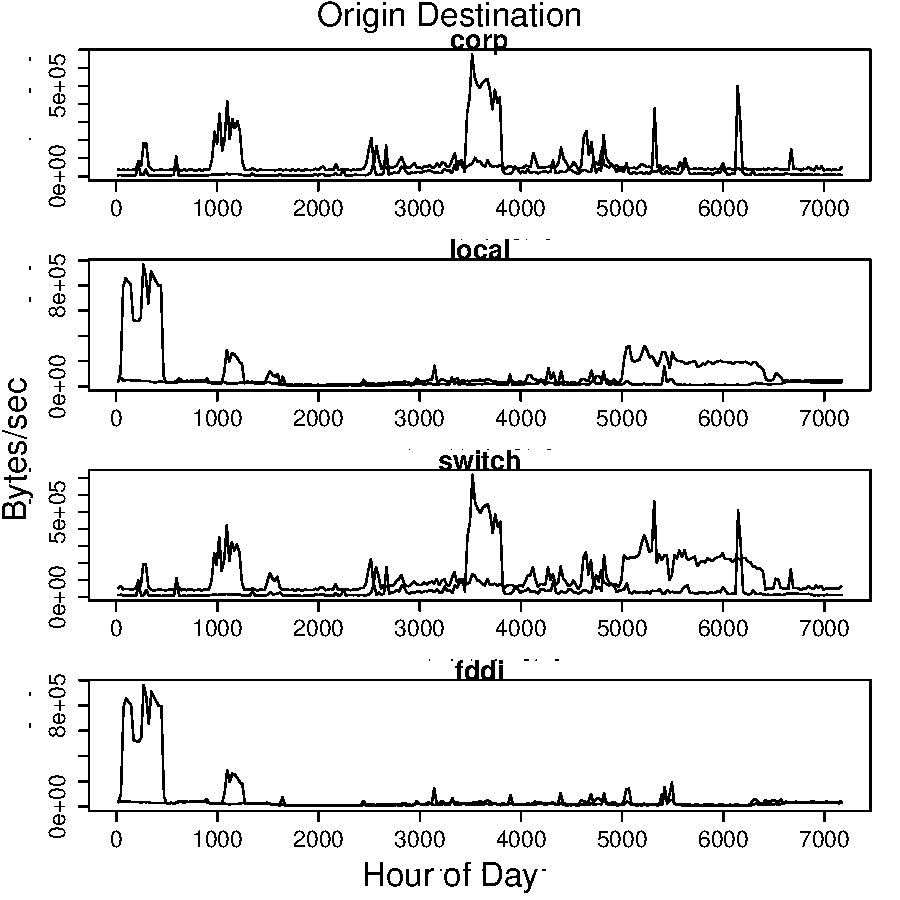
\includegraphics[scale=0.75]{tam_gregory_fig2.pdf}
\end{center}

\item 
We run the code: 
\begin{verbatimcode}
dat = read.csv("1router_allcount.dat")
attach(dat)

x.names = c("src fddi","src switch","src local","src corp","dst fddi","dst switch","dst local","dst corp")

par(mfrow=c(1,2))
means=c()
vars = c()
for(i in 1:8)
{
  means[i]=mean(value[which(nme[3301:3600]==x.names[i])+3300])
  vars[i]=var(value[which(nme[3301:3600]==x.names[i])+3300])
}
plot(log10(means),log10(vars),pch=c("1","2","3","4","5","6","7","8"),ylim=range(7,11),main="11:30")
fit=lm(log10(vars)~log10(means))
x = seq(4,6,0.1)
y = fit$coef[1] + fit$coef[2]*x
lines(x,y)

means=c()
vars = c()
for(i in 1:8)
{
  means[i]=mean(value[which(nme[4501:4800]==x.names[i])+4500])
  vars[i]=var(value[which(nme[4501:4800]==x.names[i])+4500])
}
plot(log10(means),log10(vars),pch=c("1","2","3","4","5","6","7","8"),ylim=range(7,11),main="15:30")
fit=lm(log10(vars)~log10(means))
x = seq(4,6,0.1)
y = fit$coef[1] + fit$coef[2]*x
lines(x,y)


dat2 = read.csv("2router_linkcount.dat")
attach(dat2)

x.names = c("dst router5", "dst r4-local", "dst switch", "dst r4-others","dst gw1", "dst gw2", "dst gw3", "dst gw-others", 
              "ori router5", "ori r4-local", "ori switch", "ori r4-others","ori gw1", "ori gw2", "ori gw3", "ori gw-others")

par(mfrow=c(1,2))
means=c()
vars = c()
for(i in 1:8)
{
  means[i]=mean(value[which(nme[2113:2304]==x.names[i])+2112])
  vars[i]=var(value[which(nme[2113:2304]==x.names[i])+2112])
}
plot(log10(means),log10(vars),pch=c("1","2","3","4","5","6","7","8",
                                    "9","10","11","12","13","14","15","16"),main="11:30")
fit=lm(log10(vars)~log10(means))
x = seq(2,6,0.1)
y = fit$coef[1] + fit$coef[2]*x
lines(x,y)

means=c()
vars = c()
for(i in 1:8)
{
  means[i]=mean(value[which(nme[2881:3088]==x.names[i])+2880])
  vars[i]=var(value[which(nme[2881:3088]==x.names[i])+2800])
}
plot(log10(means),log10(vars),pch=c("1","2","3","4","5","6","7","8",
                                    "9","10","11","12","13","14","15","16"),main="15:30")
fit=lm(log10(vars)~log10(means))
x = seq(2,6,0.1)
y = fit$coef[1] + fit$coef[2]*x
lines(x,y)
\end{verbatimcode}
to get the following plots:
\begin{center}
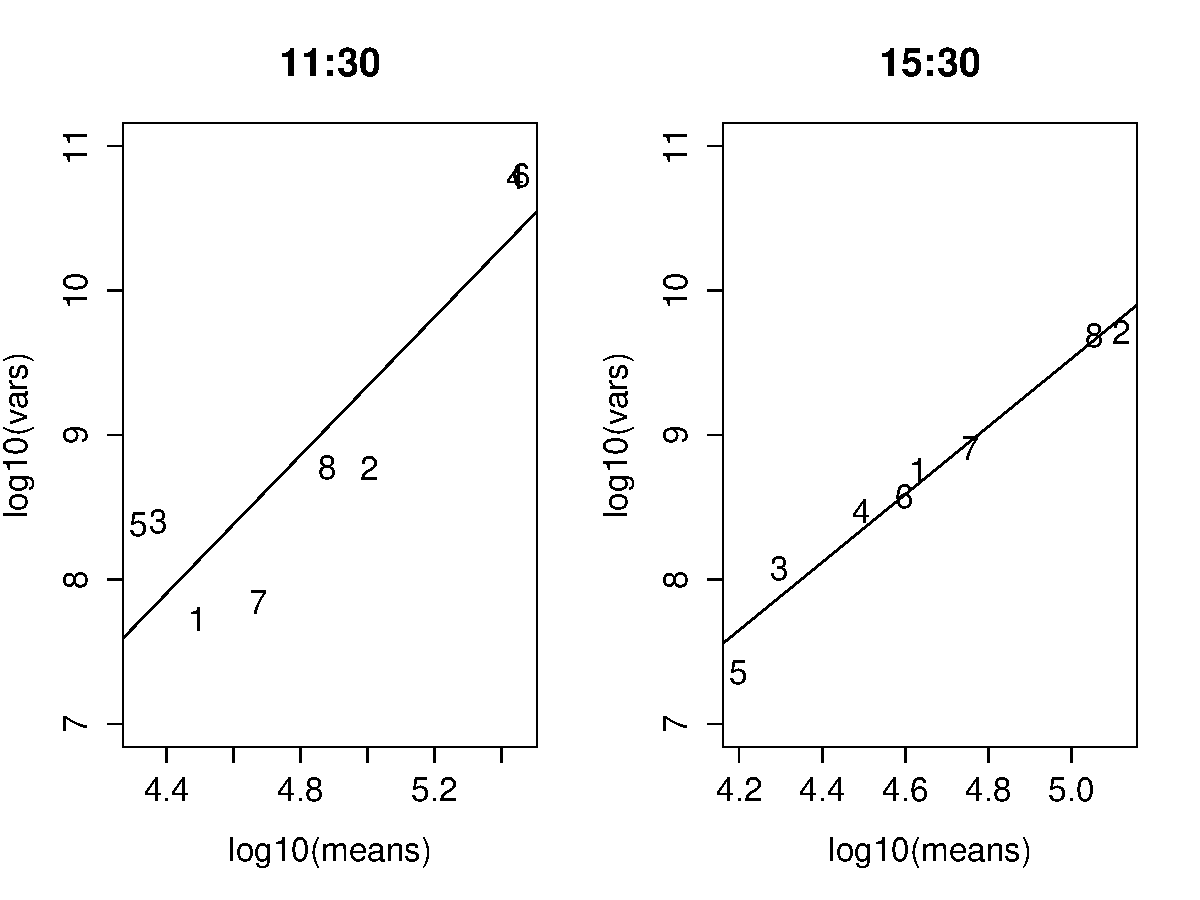
\includegraphics[scale=0.75]{tam_gregory_fig4_1router.pdf}
\end{center}
\begin{center}
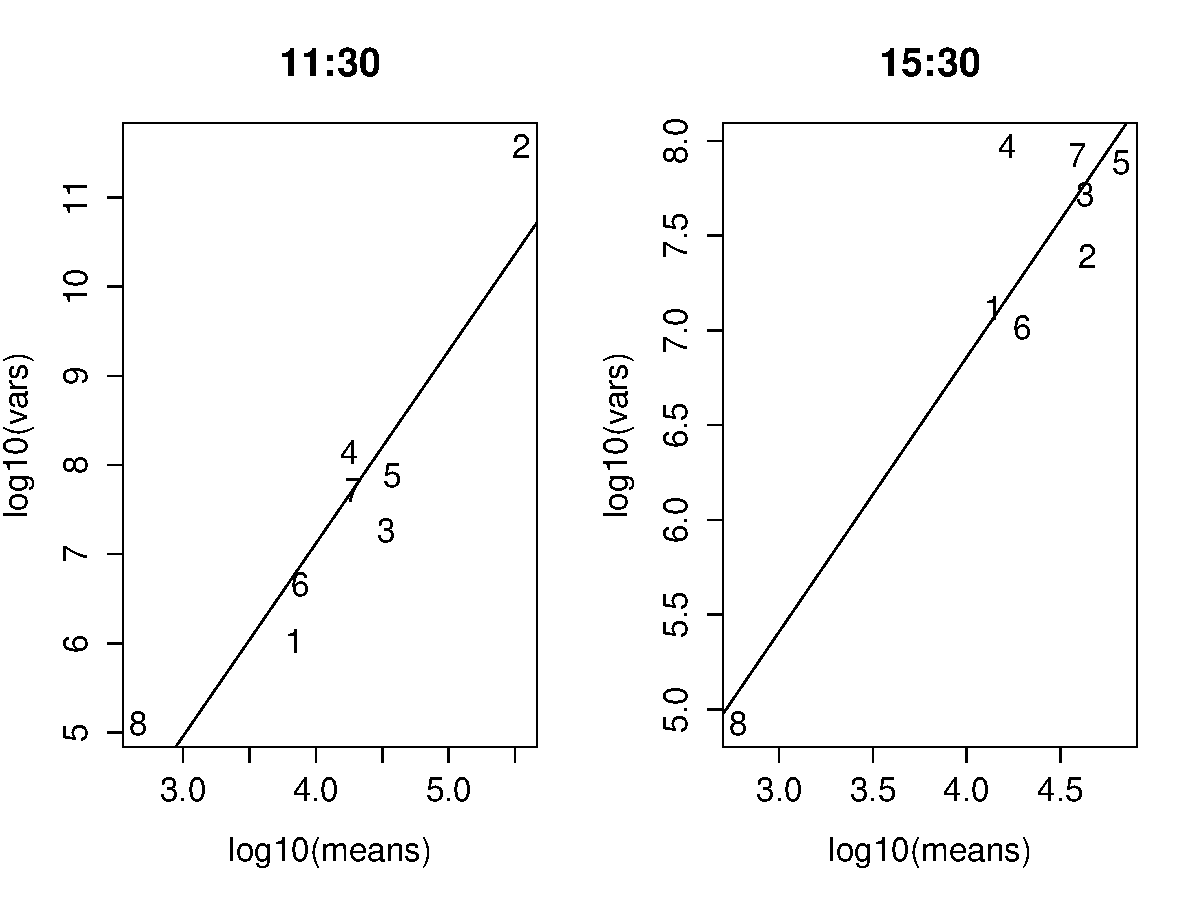
\includegraphics[scale=0.75]{tam_gregory_fig4_2router.pdf}
\end{center}

\item 
The log-likelihood of $\boldsymbol \theta | \boldsymbol X$ is
\[\ell(\boldsymbol \theta | \boldsymbol X) = -\frac{T}{2}\log | \boldsymbol \Sigma| - \frac{1}{2}\sum_{t=1}^T (\boldsymbol x_t - \boldsymbol \lambda)' \boldsymbol \Sigma^{-1} (\boldsymbol x_t - \boldsymbol \lambda) \]
To find $\E{\ell(\boldsymbol \theta | \boldsymbol X) | \boldsymbol Y, \boldsymbol \theta^{(k)}}$, we must get the distribution of $\boldsymbol x_t | \boldsymbol y_t, \boldsymbol \theta^{(k)}$.

We have that
\begin{align*}
\boldsymbol x_t | \boldsymbol \theta^{(k)} &\sim \sN(\boldsymbol \lambda^{(k)}, \boldsymbol \Sigma^{(k)})\\
\boldsymbol y_t | \boldsymbol \theta^{(k)} = \boldsymbol A \boldsymbol x_t | \boldsymbol \theta^{(k)} &\sim \sN(\boldsymbol A \boldsymbol \lambda^{(k)}, \boldsymbol A \boldsymbol \Sigma^{(k)} \boldsymbol A')
\end{align*}
We first find the joint probability, $\left.\begin{pmatrix}
\boldsymbol x_t \\ \boldsymbol y_t
\end{pmatrix} \right| \boldsymbol \theta^{(k)}$, then it is trivial to find $\boldsymbol x_t | \boldsymbol y_t, \boldsymbol \theta^{(k)}$.
As given, we have
\begin{align*}
\E{\boldsymbol x_t \middle| \boldsymbol \theta^{(k)}} &= \boldsymbol \lambda^{(k)}\\
\E{\boldsymbol y_t \middle| \boldsymbol \theta^{(k)}} &= \boldsymbol A\boldsymbol \lambda^{(k)}\\
\Var\left(\boldsymbol x_t \middle| \boldsymbol \theta^{(k)}\right) &=\boldsymbol \Sigma^{(k)}\\
\Var\left(\boldsymbol y_t \middle| \boldsymbol \theta^{(k)}\right) &= \boldsymbol A\Sigma^{(k)}\boldsymbol A'
\end{align*}
The variance-covariance matrix between $\boldsymbol x_t$ and $\boldsymbol y_t$ is
\begin{align*}
\Cov(\boldsymbol x_t, \boldsymbol y_t) &= \E{\boldsymbol x_t \boldsymbol y_t'} - \E{\boldsymbol x_t}\E{\boldsymbol y_t}'\\
&= \E{\boldsymbol x_t \boldsymbol x_t' \boldsymbol A'} - \E{\boldsymbol x_t}\E{\boldsymbol A \boldsymbol x_t}'\\
&= \E{\boldsymbol x_t \boldsymbol x_t'}\boldsymbol A' - \E{\boldsymbol x_t}\E{\boldsymbol x_t}' \boldsymbol A'\\
&= \left(\E{\boldsymbol x_t \boldsymbol x_t'}\boldsymbol  - \E{\boldsymbol x_t}\E{\boldsymbol x_t}'\right) \boldsymbol A'\\
&= \boldsymbol \Sigma^{(k)} \boldsymbol A'
\end{align*}
This gives
\[\left.\begin{pmatrix}
\boldsymbol x_t \\ 
\boldsymbol y_t
\end{pmatrix}\right | \boldsymbol \theta^{(k)} \sim \sN\left( \begin{pmatrix}
\boldsymbol \lambda^{(k)} \\ \boldsymbol A \boldsymbol \lambda^{(k)}
\end{pmatrix}, \begin{pmatrix}
\boldsymbol \Sigma^{(k)} & \boldsymbol \Sigma^{(k)} \boldsymbol A'\\
\boldsymbol A \boldsymbol \Sigma^{(k)} & \boldsymbol A \boldsymbol \Sigma^{(k)} \boldsymbol A'
\end{pmatrix}  \right) \]
Then from standard results in probability, we have
\[\boldsymbol x_t | \boldsymbol y_t, \boldsymbol \theta^{(k)} \sim \sN(\boldsymbol \lambda^{(k)} + \boldsymbol \Sigma^{(k)} \boldsymbol A' (\boldsymbol A \boldsymbol \Sigma^{(k)} \boldsymbol A')^{-1} (\boldsymbol y_t - \boldsymbol A \boldsymbol \lambda^{(k)}), \boldsymbol \Sigma^{(k)} - \boldsymbol \Sigma^{(k)}\boldsymbol A'(\boldsymbol A \boldsymbol \Sigma^{(k)} \boldsymbol A')^{-1} \boldsymbol A \boldsymbol \Sigma^{(k)}) \]
that, is we have 
\begin{align*}
\boldsymbol m_t^{(k)} &= \E{\boldsymbol x_t \middle| \boldsymbol y_t, \boldsymbol \theta^{(k)}}\\
&= \boldsymbol \lambda^{(k)} + \boldsymbol \Sigma^{(k)} \boldsymbol A' (\boldsymbol A \boldsymbol \Sigma^{(k)} \boldsymbol A')^{-1} (\boldsymbol y_t - \boldsymbol A \boldsymbol \lambda^{(k)})\\
\boldsymbol R^{(k)} &= \Var(\boldsymbol x_t | \boldsymbol y_t, \boldsymbol \theta^{(k)})\\
&=  \boldsymbol \Sigma^{(k)} - \boldsymbol \Sigma^{(k)}\boldsymbol A'(\boldsymbol A \boldsymbol \Sigma^{(k)} \boldsymbol A')^{-1} \boldsymbol A \boldsymbol \Sigma^{(k)}
\end{align*}

Now, we have
\begin{align*}
Q(\boldsymbol \theta, \boldsymbol \theta^{(k)}) &= \E{\ell(\boldsymbol \theta | \boldsymbol X) | \boldsymbol Y, \boldsymbol \theta^{(k)}}\\
&= \E{\left. -\frac{T}{2}\log | \boldsymbol \Sigma| - \frac{1}{2}\sum_{t=1}^T (\boldsymbol x_t - \boldsymbol \lambda)' \boldsymbol \Sigma^{-1} (\boldsymbol x_t - \boldsymbol \lambda) \right| \boldsymbol Y, \boldsymbol \theta^{(k)}}\\
&= \E{\left. -\frac{T}{2}\log | \boldsymbol \Sigma| \right| \boldsymbol Y, \boldsymbol \theta^{(k)}} - \E{\left.\frac{1}{2}\sum_{t=1}^T (\boldsymbol x_t - \boldsymbol \lambda)' \boldsymbol \Sigma^{-1} (\boldsymbol x_t - \boldsymbol \lambda) \right| \boldsymbol Y, \boldsymbol \theta^{(k)}}
\end{align*}
For the first term, we have
\[\E{\left. -\frac{T}{2}\log | \boldsymbol \Sigma| \right| \boldsymbol Y, \boldsymbol \theta^{(k)}} =  -\frac{T}{2}\log | \boldsymbol \Sigma|\]
as we condition on $\theta^{(k)}$, so it is constant. For the second term, we have a quadratic form. 
\begin{align*}
\E{\left.\frac{1}{2}\sum_{t=1}^T (\boldsymbol x_t - \boldsymbol \lambda)' \boldsymbol \Sigma^{-1} (\boldsymbol x_t - \boldsymbol \lambda) \right| \boldsymbol Y, \boldsymbol \theta^{(k)}} &= \E{\left.\frac{1}{2}\sum_{t=1}^T \tr\left( (\boldsymbol x_t - \boldsymbol \lambda)' \boldsymbol \Sigma^{-1} (\boldsymbol x_t - \boldsymbol \lambda) \right) \right| \boldsymbol Y, \boldsymbol \theta^{(k)}}\\
&= \E{\left.\frac{1}{2}\sum_{t=1}^T \tr\left( \boldsymbol \Sigma^{-1} (\boldsymbol x_t - \boldsymbol \lambda)(\boldsymbol x_t - \boldsymbol \lambda)'  \right) \right| \boldsymbol Y, \boldsymbol \theta^{(k)}}\\
&= \frac{1}{2}\sum_{t=1}^T \E{\tr\left(\boldsymbol \Sigma^{-1}(\boldsymbol x_t - \boldsymbol \lambda)(\boldsymbol x_t - \boldsymbol \lambda)'\right) \middle| \boldsymbol Y, \boldsymbol \theta^{(k)}}\\
&= \frac{1}{2}\sum_{t=1}^T \tr\left(\boldsymbol \Sigma^{-1} (\boldsymbol R^{(k)} + (\boldsymbol m_t^{(k)} - \boldsymbol \lambda)'\right)\\
&= \frac{1}{2}\sum_{t=1}^T \tr\left(\boldsymbol \Sigma^{-1} \boldsymbol R^{(k)} + \boldsymbol \Sigma^{-1}(\boldsymbol m_t^{(k)} - \boldsymbol \lambda)(\boldsymbol m_t^{(k)} - \boldsymbol \lambda)' \right)\\
&= \frac{1}{2}\sum_{t=1}^T \tr\left(\boldsymbol \Sigma^{-1} \boldsymbol R^{(k)}\right) + \tr\left(\boldsymbol \Sigma^{-1}(\boldsymbol m_t^{(k)} - \boldsymbol \lambda)(\boldsymbol m_t^{(k)} - \boldsymbol \lambda)' \right)\\&= \frac{1}{2}\sum_{t=1}^T \tr\left(\boldsymbol \Sigma^{-1} \boldsymbol R^{(k)}\right) + \tr\left((\boldsymbol m_t^{(k)} - \boldsymbol \lambda)'\boldsymbol \Sigma^{-1}(\boldsymbol m_t^{(k)} - \boldsymbol \lambda) \right)\\
&= \frac{T}{2}\tr\left(\boldsymbol \Sigma^{-1} \boldsymbol R^{(k)}\right) + \frac{1}{2}\sum_{t=1}^T (\boldsymbol m_t^{(k)} - \boldsymbol \lambda)'\boldsymbol \Sigma^{-1}(\boldsymbol m_t^{(k)} - \boldsymbol \lambda)
\end{align*}
Combining all this gives
\[Q(\boldsymbol \theta, \boldsymbol \theta^{(k)}) = -\frac{T}{2}\left(\log |\boldsymbol \Sigma| + \tr\left(\boldsymbol \Sigma^{-1} \boldsymbol R^{(k)}\right)\right) - \frac{1}{2}\sum_{t=1}^T  (\boldsymbol m_t^{(k)} - \boldsymbol \lambda)'\boldsymbol \Sigma^{-1}(\boldsymbol m_t^{(k)} - \boldsymbol \lambda)\]
To get $\frac{\partial Q(\boldsymbol \theta, \boldsymbol \theta^{(k)})}{\partial \boldsymbol \theta}$, we first split this up into parts, then differentiate each part. 
\begin{align*}
\frac{\partial}{\partial \lambda_i} \log |\Sigma| &=\frac{\partial}{\partial \lambda_i} \log \left| \prod_{j=1}^I \lambda_j^c \right|\\
&= \frac{c \lambda_i^{c-1}}{\prod_{j=1}^I \lambda_j^c}\\
\frac{\partial}{\partial \phi} \log | \Sigma| &= \frac{1}{\prod_{j=1}^I \lambda_j^c}
\end{align*}
For the trace term, we have
\begin{align*}
\tr(\Sigma^{-1} R^{(k)}) &= \tr \left(\begin{pmatrix}
\frac{1}{\phi \lambda_1^c} & \cdots & 0\\
\vdots & \ddots & \vdots\\
0 & \cdots & \frac{1}{\phi \lambda_I^c}
\end{pmatrix} R^{(k)} \right)\\
&= \sum_{i=1}^I  \frac{r_{ii}^{(k)}}{\phi \lambda_i^c}
\end{align*}
and so our derivatives are
\begin{align*}
\frac{\partial}{\partial \lambda_i} \tr(\Sigma^{-1} R^{(k)}) &= -\frac{cr_{ii}^{(k)}}{\phi \lambda_i^{c+1}}\\
\frac{\partial}{\partial \phi} \tr(\Sigma^{-1} R^{(k)}) &= - \sum_{i=1}^I \frac{r_{ii}^{(k)}}{\phi^2 \lambda_i^c}
\end{align*}
For the quadratic form term, we have
\begin{align*}
\sum_{t=1}^T (m_t^{(k)} - \lambda)' \Sigma^{-1}  (m_t^{(k)} - \lambda) &= \sum_{t=1}^T  (m_t^{(k)} - \lambda)' \begin{pmatrix}
\frac{1}{\phi \lambda_1^c}  (m_{t,1}^{(k)} - \lambda_1)\\
\vdots \\
\frac{1}{\phi \lambda_I^c}  (m_{t,I}^{(k)} - \lambda_I)
\end{pmatrix}\\
&= \sum_{t=1}^T \sum_{i=1}^I \frac{1}{\phi \lambda_i^c} (m_{t,i}^{(k)} - \lambda_i)^2\\
&= \sum_{t=1}^T \sum_{i=1}^I \frac{1}{\phi}\left\{\frac{(m_{t,i}^{(k)})^2}{\lambda_i^2} - \frac{2m_{t,i}^{(k)}}{\lambda_i} + 1 \right\}
\end{align*}
This gives
\begin{align*}
\frac{\partial}{\partial \lambda_i} \sum_{t=1}^T (m_t^{(k)} - \lambda)' \Sigma^{-1}  (m_t^{(k)} - \lambda)  &= \sum_{t=1}^T \sum_{i=1}^I \frac{2}{\phi}\left\{\frac{m_{t,i}^{(k)}}{\lambda_i^2} - \frac{(m_{t,i}^{(k)})^2}{\lambda_i^3}\right\}\\
\frac{\partial}{\partial \phi}\sum_{t=1}^T (m_t^{(k)} - \lambda)' \Sigma^{-1}  (m_t^{(k)} - \lambda)  &= -\sum_{t=1}^T \sum_{i=1}^I \frac{1}{\phi^2}\left\{\frac{(m_{t,i}^{(k)})^2}{\lambda_i^2} - \frac{2m_{t,i}^{(k)}}{\lambda_i} +1 \right\}
\end{align*}
Setting this to 0 will yield the equations
\begin{align*}
0 &= c \phi \lambda_i^c + (2-c)\lambda_i^2 - 2(1-c)\lambda_i b_i^{(k)} - c a_i^{(k)}\\
0 &= \sum_{i=1}^I \lambda_i^{-c+1}(\lambda_i - b_i^{(k)}
\end{align*}
where $c=2$.

\item 
In our setup, we have $\boldsymbol \theta = (\boldsymbol \lambda, \phi)$, which is a 17 dimensional vector ($\boldsymbol \lambda$ is a 16 dimensional vector and $\phi$ is a scalar. We try to find the best $\boldsymbol \theta$ given our data. At iteration $k$, we have $\boldsymbol \theta^{(k)}$, which is our current estimate of the parameter $\boldsymbol \theta$. The function that we wish to maximize at each step is $Q(\boldsymbol \theta, \boldsymbol \theta^{(k)})$ as defined above. We have that the equations $\frac{\partial Q}{\partial \theta}=0$ are equivalent to 
\begin{align*}
0 &= c \phi \lambda_i^c + (2-c)\lambda_i^2 - 2(1-c)\lambda_i b_i^{(k)} - c a_i^{(k)}\\
0 &= \sum_{i=1}^I \lambda_i^{-c+1}(\lambda_i - b_i^{(k)}
\end{align*}
as defined in the Cao, Yu paper in equation (7), therefore, all we have to do to maximize $Q(\boldsymbol \theta, \boldsymbol \theta^{(k)})$ is find the roots of the above equations. 

In our example, with $c=2$, 
\begin{align*}
0 &= c \phi \lambda_i^c + (2-c)\lambda_i^2 - 2(1-c)\lambda_i b_i^{(k)} - c a_i^{(k)}\\
&= 2 \phi \lambda_i^2 + 2 \lambda_i b_i^{(k)} - 2a_i^{(k)}
\end{align*}
which is simply a quadratic equation, so we have an analytical solution
\[\lambda_i = \frac{-b_i^{(k)} + \sqrt{{b_i^{(k)}}^2 + 4a_i^{(k)} \phi}}{2\phi} \]
where we take the positive solution since we require $\lambda_i>0$.

We start with initial values for $\boldsymbol \lambda$ and $\phi$, which are carefully chosen to the algorithm is stable. In my case, I had $\lambda_i^{(0)} = 1000000$ for each $i$ and $\phi_0=0.5$. At time step $t$, given $\phi_{t-1}$ we can solve the zeros of quadratic equation to get $\boldsymbol \lambda^{(t)}$. This saves computation time as we do not need to do any type of numerical method to find the root. Then, we need a way to get $\phi_t$ from $\boldsymbol \lambda^{(t)}$. Unfortunlately, there is no easy analytic solution that we can do as we did for $\boldsymbol \lambda$, so we do a one-step Newton-Raphson on all the parameters, but only change $\phi$ by iterating:
\[\boldsymbol \theta^{(k+1)} = \boldsymbol \theta^{(k)} - \{\dot{\boldsymbol F}(\boldsymbol \theta^{(k)})\}^{-1} \boldsymbol f(\boldsymbol \theta^{(k)}) \]
where $\dot{\boldsymbol F}$ is the Jacobian of $\boldsymbol f(\boldsymbol \theta)$ with respect to $\boldsymbol \theta$. The form of this is solved in 1.3. We iterate through these steps until convergence. Once we have these 16 plots, we can add them together to get the source and destination values for each router, as well as the total. We can do this using the following code: 
\begin{verbatimcode}
library(MASS) #ginv
dat = read.csv("1router_allcount.dat")
attach(dat)

start_time=Sys.time()

task.id = as.numeric(Sys.getenv("SLURM_ARRAY_TASK_ID"))
job.id = as.numeric(Sys.getenv("SLURM_ARRAY_JOB_ID"))

x.indices = 1:16
y.indices = 17:24
# nme[which(nme %in% nme[x.indices])]
x = matrix(value[which(nme %in% nme[x.indices])],nrow=16)
# nme[which(nme %in% nme[y.indices])]
y = matrix(value[which(nme %in% nme[y.indices])],nrow=8)

#set A matrix
I=16
J=8
c=2
T=length(nme)/25
A = matrix(,nrow=J-1,ncol=I)
rownames(A) = c("f","s","l","c","f","s","l")
A[1,]=c(rep(1,4),rep(0,12))
A[2,]=c(rep(0,4),rep(1,4),rep(0,8))
A[3,]=c(rep(0,8),rep(1,4),rep(0,4))
A[4,]=c(rep(0,12),rep(1,4))
A[5,]=rep(c(1,0,0,0),4)
A[6,]=rep(c(0,1,0,0),4)
A[7,]=rep(c(0,0,1,0),4)

ftest = function(theta,a,b,c)
{
  #the function f which we try to set to 0
  #takes theta as input, returns f(theta) vector
  ans = c()
  lambda = head(theta,length(theta)-1)
  phi = tail(theta,1)
  for(i in 1:length(theta))
  {
    if(i<=I)
      ans[i] = c*phi*lambda[i]^c + (2-c)*lambda[i]^2 - 2*(1-c)*lambda[i]*b[i] - c*a[i]
    if(i==I+1)
      ans[i] = sum(lambda^(-c+1)*(lambda - b))
  }
  ans
}

#############
#LOCAL MODEL#
#############

locally_iid_EM = function(data, c, A, lambda.init = 1e6, phi.init=0.5)
{
  w=11
  h=(w-1)/2
  T=length(nme)/25
  #initialize the theta vector for simplicity, keep all lambdas the same. 
  #choice of these parameters are important. I initially had small lambdas, and
  #the EM would not work.
  lambda = rep(lambda.init,16)
  phi = phi.init
  theta = matrix(c(lambda,phi),ncol=1)
  
  f.array = matrix(,ncol=0,nrow=I+1)
  #replicate for each t
  for(t in 6:(T-5))
  {
    #previous theta vector (lambda, phi)
    theta.old = theta[,ncol(theta)]
    theta.new=c()
    
    #E-step
    Sigma = diag(phi*lambda^c)
    min.t = t-h
    max.t = t+h
    m = sapply(min.t:max.t, function(i) lambda + Sigma %*% t(A) %*% ginv(A %*% Sigma %*% t(A)) %*% (data[-8,i] - A %*% lambda))
    R = Sigma - Sigma %*% t(A) %*% ginv(A %*% Sigma %*% t(A)) %*% A %*% Sigma
    
    #finds f, which is the derivative of Q(theta,theta^{(t)})
    #Newton-Raphson is done on f to find the maximum of Q   
    a=c()
    b=c()
    f=c()
    for(i in 1:I)
    {
      a[i] = R[i,i] + mean(m[i,]^2)
      b[i] = mean(m[i,])
      f[i] = c*phi*lambda[i]^c + (2-c)*lambda[i]^2 - 2*(1-c)*lambda[i]*b[i] - c*a[i]
    }
    f[I+1] = sum(lambda^(-c+1)*(lambda - b))
    
    
    #analytical solution: when c=2, it sets the lambda such that f()=0
    lambda = (-b + sqrt(b^2 + 4*a*phi))/(2*phi)
    #replace lambdas with analytical solutions
    theta.new[1:I] = lambda
    #check that f is close to 0
    ftest(c(lambda,phi),a,b,c)
    
    #M-step
    
    #Create Fdot matrix (derivative)
    Fdot = matrix(,nrow=I+1,ncol=I+1)
    for(i in 1:I)
      for(j in 1:I)
        Fdot[i,j] = (i==j)*(phi*c^2*lambda[i]^(c-1) + 2*(2-c)*lambda[i] - 2*(1-c)*b[i])
    for(j in 1:I)
      Fdot[I+1,j] = (2-c)*lambda[j]^(1-c) - (1-c)*lambda[j]^(-c)*b[j]
    for(i in 1:I)
      Fdot[i,I+1] = c*lambda[i]^c
    Fdot[I+1,I+1] = 0
    
    mult=1
    tempInv = ginv(Fdot) %*% f
    repeat
    {
      #Fractional Newton-Raphson: Shrinks amount it takes off to ensure phi remains greater than 0
      phi = theta.old[I+1] - mult*tempInv[I+1,]
      if(phi>0)
        break
      mult = mult/2
    }
    theta.new[I+1] = phi
    ftest(c(lambda,phi),a,b,c)

    theta.old = theta.new
    theta = cbind(theta,theta.new)
    f.array = cbind(f.array,ftest(theta.new,a,b,c))
  }
  list("f"=f.array,"theta"=theta,"a"=a,"b"=b)
}

#aggregated ftest: Since ftest is a vector, we take the sum of square since we want to minimize it
optim_ftest = function(theta,a,b,c){sum(ftest(theta,a,b,c)^2)}
Sys.time()
f_em = locally_iid_EM(y,c,A,lambda.init=1e4)


end_time = Sys.time()
total_time = as.numeric(end_time-start_time,units="mins")
save(list = c("f_em","start_time","end_time","total_time","last_par"),
               file=sprintf("odyssey/pset5/converge_task%d_job%d.rda", task.id, job.id))


#T-10 columns since we ignore the first 5 and last 5 (window size)
#ignore the first entry of theta (the -1 term) since that is our initial value.
#To find this we look at the matrix A and see which plots correspond to columns of A
theta.MA = matrix(,nrow=25,ncol=T-10)
theta.MA[6:9,] = f_em$theta[13:16,-1]
theta.MA[11:14,] = f_em$theta[9:12,-1]
theta.MA[16:19,] = f_em$theta[5:8,-1]
theta.MA[21:24,] = f_em$theta[1:4,-1]

#fill in other boxes with appropriate sums
theta.MA[1,] = apply(theta.MA[1+seq(5,20,5),],2,sum)
theta.MA[2,] = apply(theta.MA[2+seq(5,20,5),],2,sum)
theta.MA[3,] = apply(theta.MA[3+seq(5,20,5),],2,sum)
theta.MA[4,] = apply(theta.MA[4+seq(5,20,5),],2,sum)

theta.MA[10,] = apply(theta.MA[10-4:1,],2,sum)
theta.MA[15,] = apply(theta.MA[15-4:1,],2,sum)
theta.MA[20,] = apply(theta.MA[20-4:1,],2,sum)
theta.MA[25,] = apply(theta.MA[25-4:1,],2,sum)

theta.MA[5,] = apply(theta.MA[c(6:9,11:14,16:19,21:24),],2,sum)


#Plot actual data
dev.off()
par(mfrow=c(5,5),oma=c(1.5,1.5,1.5,1.5))
par(mar=c(1,1,1,0))
name.list = c("dst fddi", "dst switch", "dst local", "dst corp", "total", 
              "corp->fddi", "corp->switch", "corp->local", "corp->corp", "src corp",
              "local->fddi", "local->switch", "local->local", "local->corp", "src local",
              "switch->fddi", "switch->switch", "switch->local", "switch->corp", "src switch",
              "fddi->fddi", "fddi->switch", "fddi->local", "fddi->corp", "src fddi")
plotted.values = matrix(,nrow=25,ncol=T)
for(i in 1:25)
{
  indices = which(nme == name.list[i])
  plotted.values[i,]=value[indices]
  if(i==21) #bottom left corner
  {
    plot(plotted.values[i,],type='l',ylim=range(0,1e6),main=name.list[i],lwd=2,col="cyan")
  }else if(i>20) #bottom row
  {
    plot(plotted.values[i,],type='l',ylim=range(0,1e6),yaxt="n",main=name.list[i],lwd=2,col="cyan")
  }else if(i%%5==1) #left side
  {
    plot(plotted.values[i,],type='l',ylim=range(0,1e6),xaxt="n",main=name.list[i],lwd=2,col="cyan")
  }else #everything else (no axis labels)
  {
    plot(plotted.values[i,],type='l',ylim=range(0,1e6),xaxt="n",yaxt="n",main=name.list[i],lwd=2,col="cyan")
  }
  #Plot fitted data
  lines(1:277+5,theta.MA[i,],lwd=2)
}
\end{verbatimcode}

\begin{center}
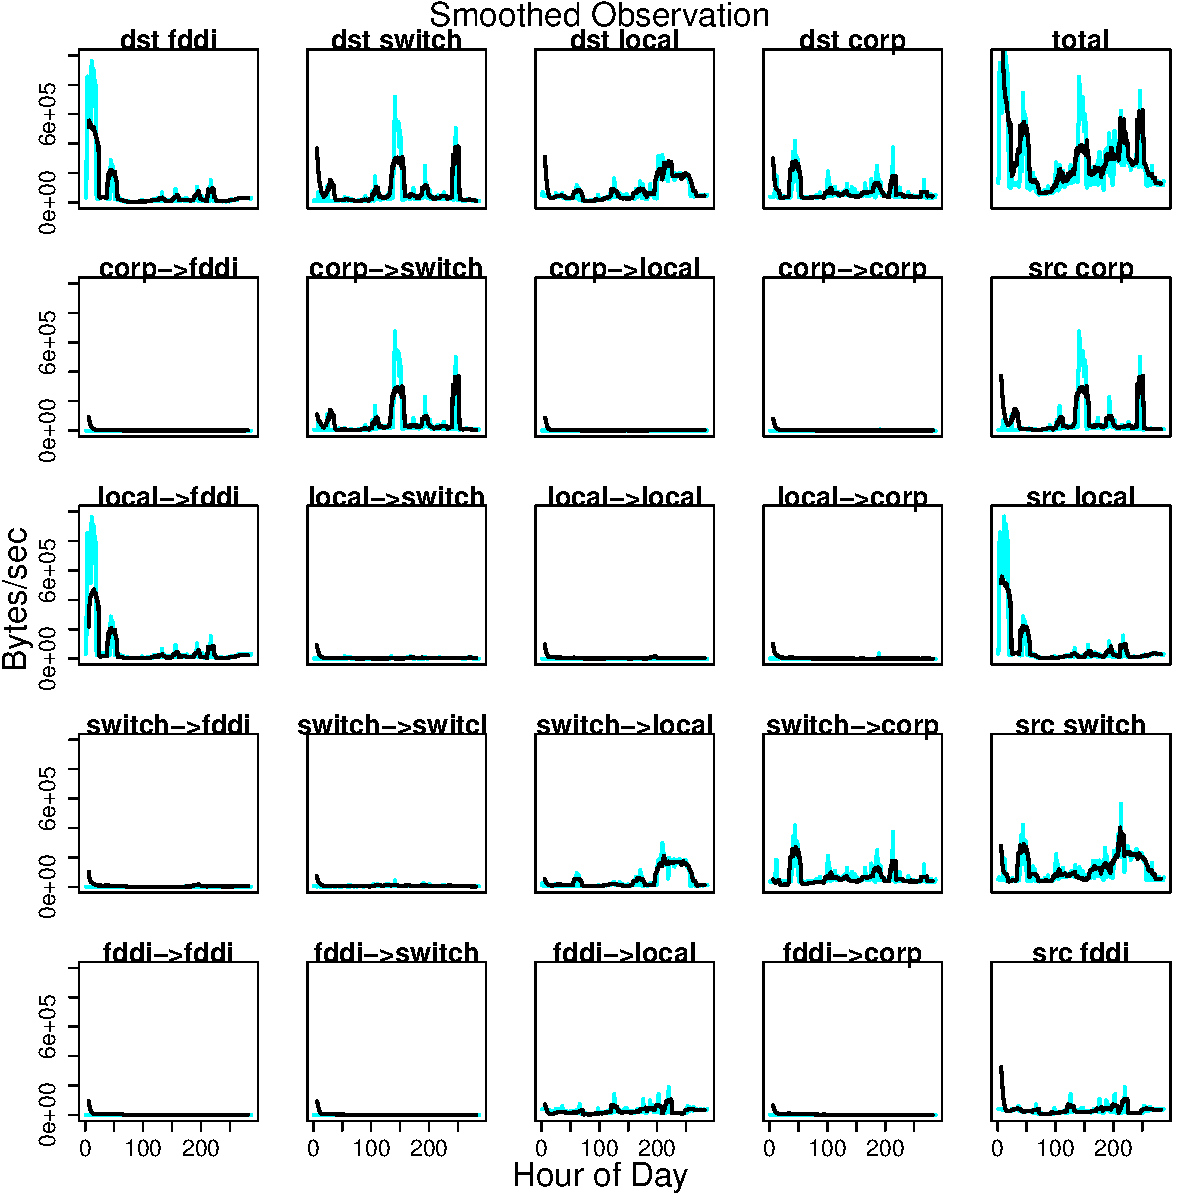
\includegraphics[scale=0.75]{tam_gregory_fig5.pdf}
\end{center}


\item 
In the smoothed case, we put additional randomness on our $\boldsymbol \theta_t$. We have 
\[\boldsymbol \eta_t = (\log \boldsymbol \lambda_t, \log \phi_t) = \log \boldsymbol \theta_t\]
To maintain consistent notation with the paper, we have $\tilde{\boldsymbol Y}_t = (\boldsymbol y_1,\ldots,\boldsymbol y_{t+h})$ and $\boldsymbol Y_t = (\boldsymbol y_{t-h},\ldots,\boldsymbol y_{t+h})$. As before, the likelihood is given by
\[\ell(\boldsymbol \eta_t | \boldsymbol X) =  -\frac{w}{2}\log | \boldsymbol \Sigma_t| - \frac{1}{2}\sum_{i=t-h}^{t+h} (\boldsymbol x_i - \boldsymbol \lambda_t)' \boldsymbol \Sigma_t^{-1} (\boldsymbol x_i - \boldsymbol \lambda_t) \]
where now, instead of summing from $i=1,\ldots,T$, we sum $i=t-h,\ldots,t,\ldots,t+h$ because this is 
a local model. 

In the smoothed case, since $\boldsymbol \theta_t$, and by extension, $\boldsymbol \eta_t$ are random, we have an added prior, given $\tilde{\boldsymbol Y}_t = (\boldsymbol y_1,\ldots,\boldsymbol y_{t+h})$.
In the Cao and Yu paper on page 1071, a Normal approximation to the prior is given by
\[ \pi(\boldsymbol \eta_t | \tilde{\boldsymbol Y}_t) \approx \sN(\hat{\boldsymbol \eta}_{t-1}, \hat{\boldsymbol \Sigma}_{t-1} + \boldsymbol V) \]
where $\hat{\boldsymbol \eta}_{t-1}$ is the posterior mode and $\hat{\boldsymbol \Sigma}_{t-1}$ is the inverse of the curvature of the log posterior density at the mode. We know this since we have
\[\boldsymbol \eta_t = \boldsymbol \eta_{t-1} + \boldsymbol v_t, \qquad \boldsymbol v_t \sim \sN(\boldsymbol 0,\boldsymbol V)\]
then
\[\boldsymbol \eta_t | \boldsymbol \eta_{t-1} \sim \sN(\boldsymbol \eta_{t-1}, \boldsymbol V)\]
We also know that
\[\boldsymbol \eta_{t-1} | \tilde{\boldsymbol Y}_{t-1} \approx \sN(\hat{\boldsymbol \eta}_{t-1}, \hat{\boldsymbol \Sigma}_{t-1})\]
This gives
\begin{align*}
\boldsymbol \eta_t | \tilde{\boldsymbol Y}_{t-1} &= \boldsymbol \eta_{t-1}| \tilde{\boldsymbol Y}_{t-1} + \boldsymbol v_t | \tilde{\boldsymbol Y}_{t-1}\\
&\sim \sN(\hat{\boldsymbol \eta}_{t-1}, \hat{\boldsymbol  \Sigma}_{t-1}) + \sN(\boldsymbol 0, \boldsymbol V)\\
&\sim \sN(\hat{\boldsymbol \eta}_{t-1}, \hat{\boldsymbol \Sigma}_{t-1} + \boldsymbol V )
\end{align*}

We wish to maximize 
\[g(\boldsymbol \eta_t) = \log \pi(\boldsymbol \eta_t) + \log \p{\tilde{\boldsymbol Y}_t | \boldsymbol \eta_t}\]
As before, we can bound this by
\[Q(\boldsymbol \theta, \boldsymbol \theta^{(k)}) =  \log \pi(\boldsymbol \eta_t) + Q_{local}(\boldsymbol \theta, \boldsymbol \theta^{(k)}) \]
where $Q_{local}(\boldsymbol \theta, \boldsymbol \theta^{(k)}) $ is the same $Q$ function in the iid case. Thus, only our M step is changed via this modified $Q$ function.


\item Fitting the refined model only differs in the $Q(\boldsymbol \theta, \boldsymbol \theta^{(k)})$ function. However, in practice, this becomes a bit more difficult. In the local i.i.d. case, we could maximize $Q(\boldsymbol \theta, \boldsymbol \theta^{(k)})$ by solving for
\begin{align*}
0 &= c \phi \lambda_i^c + (2-c)\lambda_i^2 - 2(1-c) \lambda_i b_i^{(k)} - c a_i^{(k)}\\
0 &= \sum_{i=1}^I \lambda_i^{-c+1} (\lambda_i - b_i^{(k)})
\end{align*}
Because the $Q$ function for the smoothed case has the extra log-prior term, solving this will not lead to the same results. We now need to solve for $\frac{\partial Q}{\partial \boldsymbol \theta}=0$ numerically. Using \texttt{optim} over all $\eta_i$ parameters did not yield any change. Instead, we change it to coordinate-wise, that is fix all $\eta_j$, $j \neq i$ and optimize $\eta_i$. We then repeat this for all $i$ and repeat the entire process for an arbitrary amount until convergence is achieved. We run the following code: 

\begin{verbatimcode}
library(numDeriv) #hessian function
library(mvtnorm)
library(psych) #trace function
library(MASS) #ginnv

dlogprior = function(eta,eta.hat,Sigma.hat)
{
  dmvnorm(eta, mean=eta.hat, sigma=Sigma.hat, log=TRUE)
}
dloglikelihood = function(Y,A,lambda,Sigma)
{
  dmvnorm(Y, mean=A %*% lambda, sigma= A %*% Sigma %*% t(A), log=TRUE)
}

library(MASS) #ginv
dat = read.csv("1router_allcount.dat")
attach(dat)

start_time=Sys.time()

task.id = as.numeric(Sys.getenv("SLURM_ARRAY_TASK_ID"))
job.id = as.numeric(Sys.getenv("SLURM_ARRAY_JOB_ID"))

x.indices = 1:16
y.indices = 17:24
# nme[which(nme %in% nme[x.indices])]
x = matrix(value[which(nme %in% nme[x.indices])],nrow=16)
# nme[which(nme %in% nme[y.indices])]
y = matrix(value[which(nme %in% nme[y.indices])],nrow=8)




I=16
J=8
c=2
T=length(nme)/25
A = matrix(,nrow=J-1,ncol=I)
rownames(A) = c("f","s","l","c","f","s","l")
A[1,]=c(rep(1,4),rep(0,12))
A[2,]=c(rep(0,4),rep(1,4),rep(0,8))
A[3,]=c(rep(0,8),rep(1,4),rep(0,4))
A[4,]=c(rep(0,12),rep(1,4))
A[5,]=rep(c(1,0,0,0),4)
A[6,]=rep(c(0,1,0,0),4)
A[7,]=rep(c(0,0,1,0),4)



#Step 2
smoothed_EM = function(data,c,A,V.init,eta.init)
{
  I=ncol(A)
  J=nrow(A)+1
  c=2
  
  #Step 1 (Set initial parameters)
  h=5
  w=2*h+1
  t=h+1
  eta = matrix(rep(eta.init,17),nrow=17,ncol=1)
  V = diag(rep(V.init,17))
  f.array = matrix(,ncol=0,nrow=I+1)


  #Step 2
  for(t in 6:(T-5))
  {
    eta.hat.old = eta[,ncol(eta)]
    eta.hat.new = c()
    
    #E-step
    #set lambda and phi based on eta
    lambda = exp(head(eta.hat.old,length(eta.hat.old)-1))
    phi = exp(tail(eta.hat.old,1))
    
    Sigma.full = diag(c(phi*lambda^c, phi))
    Sigma = diag(phi*lambda^c)
    min.t = t-h
    max.t = t+h
    m = sapply(min.t:max.t, function(i) lambda + Sigma %*% t(A) %*% ginv(A %*% Sigma %*% t(A)) %*% (data[-8,i] - A %*% lambda))
    R = Sigma - Sigma %*% t(A) %*% ginv(A %*% Sigma %*% t(A)) %*% A %*% Sigma
    
    Q.local = -w/2*(log(det(Sigma))) + tr(ginv(Sigma) %*% R) - 1/2*sum(sapply(1:11,function(i) t(m[,i]-lambda) %*% ginv(Sigma) %*% (m[,i]-lambda)))  
    Q.prior = function(eta.val)
    {
      eta.hat.old
      Sigma.hat = Sigma.full + V
      dmvnorm(eta.val, mean=eta.hat.old, sigma=Sigma.hat, log=TRUE)
    }
    g = function(eta.val){Q.local + Q.prior(eta.val)}
    
    #Find mode of g
    #Optimizing over all eta's at once doesn't work, so we do it termwise
    g.marginal = function(eta.change, eta.val,index)
    {
      #eta.change: eta coordinate we change
      #index: index for eta.change
      #eta.val: vector of etas
      eta.val[index]=eta.change
      g(eta.val)
    }
    
    eta.hat.new=eta.hat.old
    eta.hat.new[1] = optim(1, g.marginal, eta.val=eta.hat.old, index=1, control=list(fnscale=-1),method="Brent",lower=1.0001,upper=1e7)$par
    for(reps in 1:20)
    {
      for(i in 1:17)
      {
        eta.hat.new[i] = optim(eta.hat.new[i], g.marginal, eta.val=eta.hat.new, index=i, control=list(fnscale=-1),method="Brent",
                                  lower=1.0001,upper=1e7)$par
      }
    }
    eta.hat.old = eta.hat.new
    eta = cbind(eta,eta.hat.new)
    f.array = cbind(f.array,exp(dlogprior(head(eta.hat.new,length(eta.hat.new)-1),head(eta.hat.old,length(eta.hat.old)-1),Sigma) + 
                dloglikelihood(t(data[-8,t]),A,lambda,Sigma)))
    print(paste("Step",t))
  }
  list("f"=f.array,"eta"=eta, "theta"=exp(eta))
}

f_em = smoothed_EM(y,c,A,V.init=100,eta.init=11)


#T-10 columns since we ignore the first 5 and last 5 (window size)
#ignore the first entry of theta (the -1 term) since that is our initial value.
#To find this we look at the matrix A and see which plots correspond to columns of A
theta.MA = matrix(,nrow=25,ncol=T-10)
theta.MA[6:9,] = f_em$theta[13:16,-1]
theta.MA[11:14,] = f_em$theta[9:12,-1]
theta.MA[16:19,] = f_em$theta[5:8,-1]
theta.MA[21:24,] = f_em$theta[1:4,-1]

#fill in other boxes with appropriate sums
theta.MA[1,] = apply(theta.MA[1+seq(5,20,5),],2,sum)
theta.MA[2,] = apply(theta.MA[2+seq(5,20,5),],2,sum)
theta.MA[3,] = apply(theta.MA[3+seq(5,20,5),],2,sum)
theta.MA[4,] = apply(theta.MA[4+seq(5,20,5),],2,sum)

theta.MA[10,] = apply(theta.MA[10-4:1,],2,sum)
theta.MA[15,] = apply(theta.MA[15-4:1,],2,sum)
theta.MA[20,] = apply(theta.MA[20-4:1,],2,sum)
theta.MA[25,] = apply(theta.MA[25-4:1,],2,sum)

theta.MA[5,] = apply(theta.MA[c(6:9,11:14,16:19,21:24),],2,sum)




dev.off()
par(mfrow=c(5,5),oma=c(1.5,1.5,1.5,1.5))
par(mar=c(2.5,2.5,1,0))
name.list = c("dst fddi", "dst switch", "dst local", "dst corp", "total", 
              "corp->fddi", "corp->switch", "corp->local", "corp->corp", "src corp",
              "local->fddi", "local->switch", "local->local", "local->corp", "src local",
              "switch->fddi", "switch->switch", "switch->local", "switch->corp", "src switch",
              "fddi->fddi", "fddi->switch", "fddi->local", "fddi->corp", "src fddi")
plotted.values = matrix(,nrow=25,ncol=T)
for(i in 1:25)
{
  indices = which(nme == name.list[i])
  plotted.values[i,]=value[indices]
  if(i==21) #bottom left corner
  {
    plot(plotted.values[i,],type='l',ylim=range(0,1e6),main=name.list[i],lwd=2,col="cyan")
  }else if(i>20) #bottom row
  {
    plot(plotted.values[i,],type='l',ylim=range(0,1e6),yaxt="n",main=name.list[i],lwd=2,col="cyan")
  }else if(i%%5==1) #left side
  {
    plot(plotted.values[i,],type='l',ylim=range(0,1e6),xaxt="n",main=name.list[i],lwd=2,col="cyan")
  }else #everything else (no axis labels)
  {
    plot(plotted.values[i,],type='l',ylim=range(0,1e6),xaxt="n",yaxt="n",main=name.list[i],lwd=2,col="cyan")
  }
  #Plot fitted data
  lines(1:277+5,theta.MA[i,],lwd=2)
}

mtext("Smoothed Observation",outer=TRUE)
mtext("Bytes/sec",outer=TRUE,side=2)
mtext("Hour of Day",outer=TRUE,side=1)
\end{verbatimcode}
\begin{center}
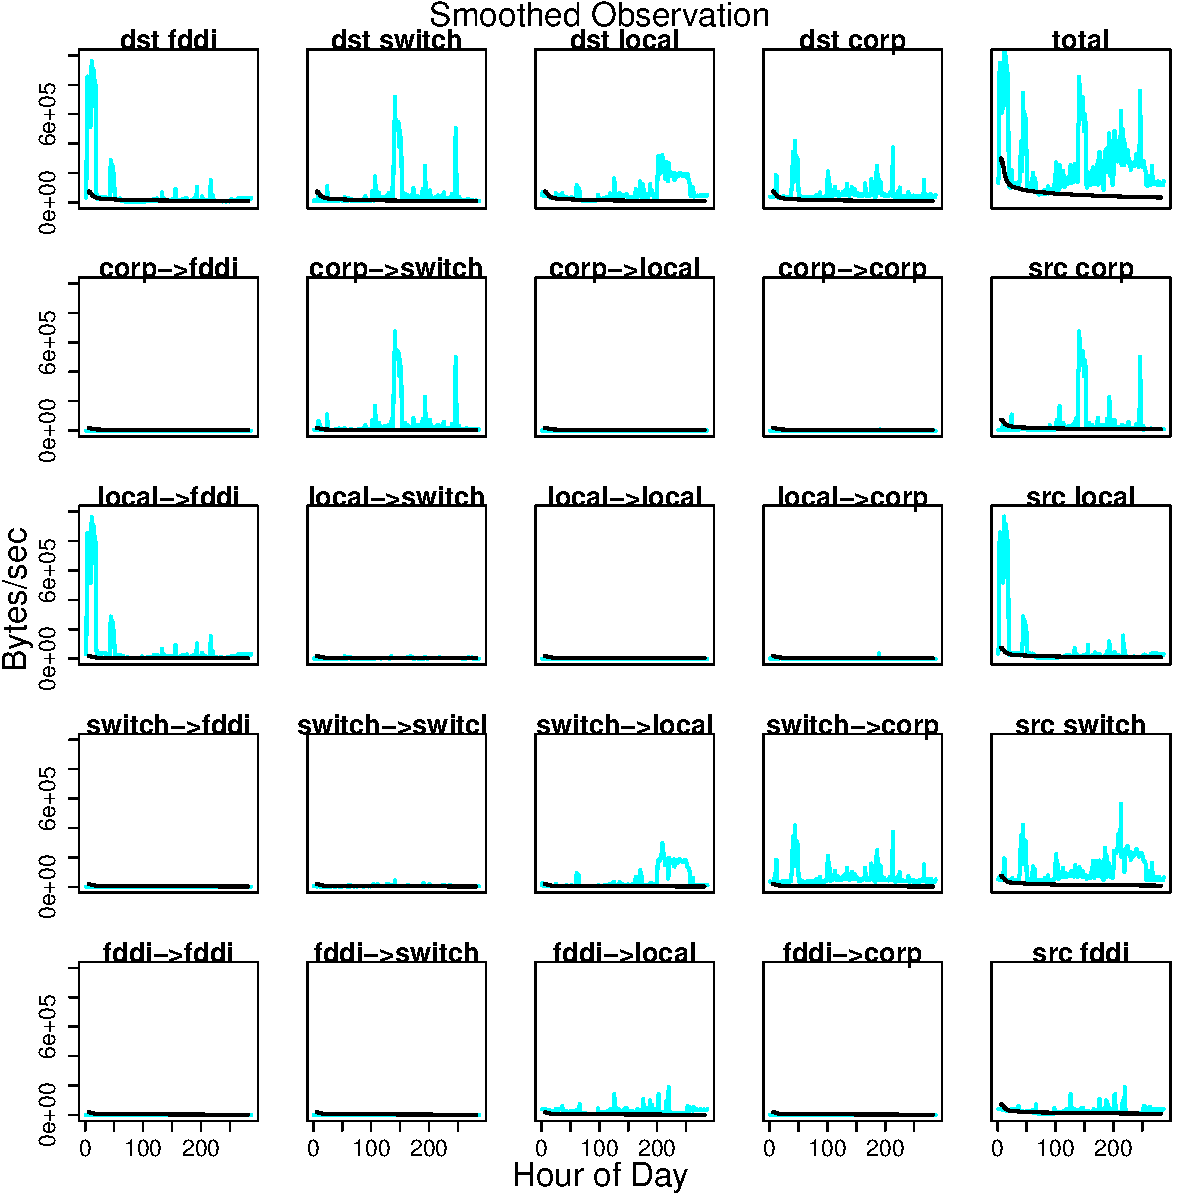
\includegraphics[scale=0.75]{tam_gregory_fig6_1router.pdf}
\end{center}


\item There is no question 1.7

\item
Two of the models outlined in Cao and Yu's paper are an i.i.d. model with fixed, unknown parameters $\lambda, \phi$ and the local i.i.d. model with $\eta_t$ as a Normal random variable and moving windows. 

The methods suggested in Tebaldi and West also implements a Bayesian perspective, that is where $\lambda_t$, or equivalently, $\eta_t$ have a prior, but instead of dealing with a window of link counts, only looks at a single one. By doing this, it removes some of the dependency and smoothing structure of the window of link counts. We should then expect the local i.i.d. method presented by Cao and Yu to outperform that of Tebaldi and West.

\item When looking at the data in \texttt{2router\_linkcount.dat}, we have 8 different routers. We will have $9 \times 9 = 81$ plots. In this case, we only know $y$, that is only the observed variables and not the latent ones $x$. So, we can only plot the estimates for the unobserved OD byte counts.

\begin{verbatimcode}
library(MASS) #ginv
dat = read.csv("2router_linkcount.dat")
attach(dat)

start_time=Sys.time()

task.id = as.numeric(Sys.getenv("SLURM_ARRAY_TASK_ID"))
job.id = as.numeric(Sys.getenv("SLURM_ARRAY_JOB_ID"))

y = matrix(value[which(nme %in% nme[1:16])],nrow=16)



#set A matrix
I=64
J=16
c=2
T=length(nme)/16
A = matrix(,nrow=J-1,ncol=I)
rownames(A) = c("router5","r4-local","switch","r4-others","gw1","gw2","gw3","gw-others","router5","r4-local","switch","r4-others","gw1","gw2","gw3")
A[1,]=c(rep(1,8),rep(0,56))
A[2,]=c(rep(0,8),rep(1,8),rep(0,48))
A[3,]=c(rep(0,16),rep(1,8),rep(0,40))
A[4,]=c(rep(0,24),rep(1,8),rep(0,32))
A[5,]=c(rep(0,32),rep(1,8),rep(0,24))
A[6,]=c(rep(0,40),rep(1,8),rep(0,16))
A[7,]=c(rep(0,48),rep(1,8),rep(0,8))
A[8,]=c(rep(0,56),rep(1,8))
A[9,]=rep(c(1,0,0,0,0,0,0,0),4)
A[10,]=rep(c(0,1,0,0,0,0,0,0),4)
A[11,]=rep(c(0,0,1,0,0,0,0,0),4)
A[12,]=rep(c(0,0,0,1,0,0,0,0),4)
A[13,]=rep(c(0,0,0,0,1,0,0,0),4)
A[14,]=rep(c(0,0,0,0,0,1,0,0),4)
A[15,]=rep(c(0,0,0,0,0,0,1,0),4)

ftest = function(theta,a,b,c)
{
  #the function f which we try to set to 0
  #takes theta as input, returns f(theta) vector
  ans = c()
  lambda = head(theta,length(theta)-1)
  phi = tail(theta,1)
  for(i in 1:length(theta))
  {
    if(i<=I)
      ans[i] = c*phi*lambda[i]^c + (2-c)*lambda[i]^2 - 2*(1-c)*lambda[i]*b[i] - c*a[i]
    if(i==I+1)
      ans[i] = sum(lambda^(-c+1)*(lambda - b))
  }
  ans
}

#############
#LOCAL MODEL#
#############

locally_iid_EM = function(data, c, A, lambda.init = 1e6, phi.init=0.5)
{
  w=11
  h=(w-1)/2
  T=length(nme)/16
  #initialize the theta vector for simplicity, keep all lambdas the same. 
  #choice of these parameters are important. I initially had small lambdas, and
  #the EM would not work.
  lambda = rep(lambda.init,64)
  phi = phi.init
  theta = matrix(c(lambda,phi),ncol=1)
  
  f.array = matrix(,ncol=0,nrow=I+1)
  #replicate for each t
  for(t in 6:(T-5))
  {
    #previous theta vector (lambda, phi)
    theta.old = theta[,ncol(theta)]
    theta.new=c()
    
    #E-step
    Sigma = diag(phi*lambda^c)
    min.t = t-h
    max.t = t+h
    m = sapply(min.t:max.t, function(i) lambda + Sigma %*% t(A) %*% ginv(A %*% Sigma %*% t(A)) %*% (data[-16,i] - A %*% lambda))
    R = Sigma - Sigma %*% t(A) %*% ginv(A %*% Sigma %*% t(A)) %*% A %*% Sigma
    
    #finds f, which is the derivative of Q(theta,theta^{(t)})
    #Newton-Raphson is done on f to find the maximum of Q   
    a=c()
    b=c()
    f=c()
    for(i in 1:I)
    {
      a[i] = R[i,i] + mean(m[i,]^2)
      b[i] = mean(m[i,])
      f[i] = c*phi*lambda[i]^c + (2-c)*lambda[i]^2 - 2*(1-c)*lambda[i]*b[i] - c*a[i]
    }
    f[I+1] = sum(lambda^(-c+1)*(lambda - b))
    
    
    #analytical solution: when c=2, it sets the lambda such that f()=0
    lambda = (-b + sqrt(b^2 + 4*a*phi))/(2*phi)
    #replace lambdas with analytical solutions
    theta.new[1:I] = lambda
    #check that f is close to 0
    ftest(c(lambda,phi),a,b,c)
    
    #M-step
    
    #Create Fdot matrix (derivative)
    Fdot = matrix(,nrow=I+1,ncol=I+1)
    for(i in 1:I)
      for(j in 1:I)
        Fdot[i,j] = (i==j)*(phi*c^2*lambda[i]^(c-1) + 2*(2-c)*lambda[i] - 2*(1-c)*b[i])
    for(j in 1:I)
      Fdot[I+1,j] = (2-c)*lambda[j]^(1-c) - (1-c)*lambda[j]^(-c)*b[j]
    for(i in 1:I)
      Fdot[i,I+1] = c*lambda[i]^c
    Fdot[I+1,I+1] = 0
    
    mult=1
    tempInv = ginv(Fdot) %*% f
    repeat
    {
      #Fractional Newton-Raphson: Shrinks amount it takes off to ensure phi remains greater than 0
      phi = theta.old[I+1] - mult*tempInv[I+1,]
      if(phi>0)
        break
      mult = mult/2
    }
    theta.new[I+1] = phi
    ftest(c(lambda,phi),a,b,c)
    
    theta.old = theta.new
    theta = cbind(theta,theta.new)
    f.array = cbind(f.array,ftest(theta.new,a,b,c))
  }
  list("f"=f.array,"theta"=theta,"a"=a,"b"=b)
}

#aggregated ftest: Since ftest is a vector, we take the sum of square since we want to minimize it
optim_ftest = function(theta,a,b,c){sum(ftest(theta,a,b,c)^2)}
Sys.time()
f_em = locally_iid_EM(y,c,A,lambda.init=1e4)
f_em$f


end_time = Sys.time()
total_time = as.numeric(end_time-start_time,units="mins")
save(list = c("f_em","start_time","end_time","total_time","last_par"), file=sprintf("odyssey/pset5/converge_task%d_job%d.rda", task.id, job.id))


#T-10 columns since we ignore the first 5 and last 5 (window size)
#ignore the first entry of theta (the -1 term) since that is our initial value.
#To find this we look at the matrix A and see which plots correspond to columns of A
theta.MA = matrix(,nrow=81,ncol=T-10)

theta.MA[10:17,] = f_em$theta[13:16,-1]
theta.MA[9+10:17,] = f_em$theta[9:12,-1]
theta.MA[9*2+10:17,] = f_em$theta[5:8,-1]
theta.MA[9*3+10:17,] = f_em$theta[1:4,-1]
theta.MA[9*4+10:17,] = f_em$theta[13:16,-1]
theta.MA[9*5+10:17,] = f_em$theta[9:12,-1]
theta.MA[9*6+10:17,] = f_em$theta[5:8,-1]
theta.MA[9*7+10:17,] = f_em$theta[1:4,-1]

#fill in other boxes with appropriate sums
theta.MA[1,] = apply(theta.MA[1+seq(9,72,9),],2,sum)
theta.MA[2,] = apply(theta.MA[2+seq(9,72,9),],2,sum)
theta.MA[3,] = apply(theta.MA[3+seq(9,72,9),],2,sum)
theta.MA[4,] = apply(theta.MA[4+seq(9,72,9),],2,sum)
theta.MA[5,] = apply(theta.MA[5+seq(9,72,9),],2,sum)
theta.MA[6,] = apply(theta.MA[6+seq(9,72,9),],2,sum)
theta.MA[7,] = apply(theta.MA[7+seq(9,72,9),],2,sum)
theta.MA[8,] = apply(theta.MA[8+seq(9,72,9),],2,sum)

theta.MA[18,] = apply(theta.MA[18-8:1,],2,sum)
theta.MA[27,] = apply(theta.MA[27-8:1,],2,sum)
theta.MA[36,] = apply(theta.MA[36-8:1,],2,sum)
theta.MA[45,] = apply(theta.MA[45-8:1,],2,sum)
theta.MA[54,] = apply(theta.MA[54-8:1,],2,sum)
theta.MA[63,] = apply(theta.MA[63-8:1,],2,sum)
theta.MA[72,] = apply(theta.MA[72-8:1,],2,sum)
theta.MA[81,] = apply(theta.MA[80-8:1,],2,sum)

theta.MA[9,] = apply(theta.MA[c(10:17,19:26,28:35,37:44,46:53,55:62,64:71,73:79),],2,sum)


#Plot actual data
dev.off()
pdf("tam_gregory_fig6_2router.pdf",width=9,height=9)
par(mfrow=c(9,9),oma=c(1.5,1.5,1.5,1.5))
par(mar=c(2.5,2.5,1,0))
name.list = c("dst router5", "dst r4-local", "dst switch", "dst r4-others","dst gw1", "dst gw2", "dst gw3", "dst gw-others", 
              "ori router5", "ori r4-local", "ori switch", "ori r4-others","ori gw1", "ori gw2", "ori gw3", "ori gw-others")
plotted.values = matrix(,nrow=81,ncol=T)

#stores indices of destimation and origin values so we know for which values of i to plot
index_vec = c(1:8,seq(18,81,9))
for(i in 1:81)
{
  if(i %in% index_vec)
  {
    indices = which(nme == name.list[which(index_vec==i)])
    plotted.values[i,]=value[indices]
    if(i==1)
    {
      plot(plotted.values[i,],type='l',ylim=range(0,1e6),xaxt="n",main=name.list[which(index_vec==i)],lwd=2,col="cyan")
    }else if(i==81)
    {
      plot(plotted.values[i,],type='l',ylim=range(0,1e6),yaxt="n",main=name.list[which(index_vec==i)],lwd=2,col="cyan")
    }else
    {
      plot(plotted.values[i,],type='l',ylim=range(0,1e6),xaxt="n",yaxt="n",main=name.list[which(index_vec==i)],lwd=2,col="cyan")
    }
  }else if(i==73) #bottom left corner
  {
    plot(-1,type='l',xlim=range(1,288),ylim=range(0,1e6),main=name.list[i],lwd=2,col="cyan")
  }else if(i>73) #bottom row
  {
    plot(-1,type='l',xlim=range(1,288),ylim=range(0,1e6),yaxt="n",lwd=2,col="cyan")
  }else if(i%%9==1) #left side
  {
    plot(-1,type='l',xlim=range(1,288),ylim=range(0,1e6),xaxt="n",lwd=2,col="cyan")
  }else #everything else (no axis labels)
  {
    plot(-1,type='l',xlim=range(1,288),ylim=range(0,1e6),xaxt="n",yaxt="n",lwd=2,col="cyan")
  }
  #Plot fitted data
  lines(1:278+5,theta.MA[i,],lwd=2)
}
mtext("Local Observation",outer=TRUE)
mtext("Bytes/sec",outer=TRUE,side=2)
mtext("Hour of Day",outer=TRUE,side=1)
dev.off()







################
#SMOOTHED MODEL#
################

smoothed_EM = function(data,c,A,V.init,eta.init)
{
  I=ncol(A)
  J=nrow(A)+1
  c=2
  
  #Step 1 (Set initial parameters)
  h=5
  w=2*h+1
  t=h+1
  eta = matrix(rep(eta.init,65),nrow=65,ncol=1)
  V = diag(rep(V.init,65))
  f.array = matrix(,ncol=0,nrow=I+1)
  
  
  #Step 2
  for(t in 6:(T-5))
  {
    eta.hat.old = eta[,ncol(eta)]
    eta.hat.new = c()
    
    #E-step
    #set lambda and phi based on eta
    lambda = exp(head(eta.hat.old,length(eta.hat.old)-1))
    phi = exp(tail(eta.hat.old,1))
    
    Sigma.full = diag(c(phi*lambda^c, phi))
    Sigma = diag(phi*lambda^c)
    min.t = t-h
    max.t = t+h
    m = sapply(min.t:max.t, function(i) lambda + Sigma %*% t(A) %*% ginv(A %*% Sigma %*% t(A)) %*% (data[-16,i] - A %*% lambda))
    R = Sigma - Sigma %*% t(A) %*% ginv(A %*% Sigma %*% t(A)) %*% A %*% Sigma
    
    Q.local = -w/2*(log(det(Sigma))) + tr(ginv(Sigma) %*% R) - 1/2*sum(sapply(1:11,function(i) t(m[,i]-lambda) %*% ginv(Sigma) %*% (m[,i]-lambda)))  
    Q.prior = function(eta.val)
    {
      eta.hat.old
      Sigma.hat = Sigma.full + V
      dmvnorm(eta.val, mean=eta.hat.old, sigma=Sigma.hat, log=TRUE)
    }
    g = function(eta.val){Q.local + Q.prior(eta.val)}
    
    #Find mode of g
    #Optimizing over all eta's at once doesn't work, so we do it termwise
    g.marginal = function(eta.change, eta.val,index)
    {
      #eta.change: eta coordinate we change
      #index: index for eta.change
      #eta.val: vector of etas
      eta.val[index]=eta.change
      g(eta.val)
    }
    
    eta.hat.new=eta.hat.old
    eta.hat.new[1] = optim(1, g.marginal, eta.val=eta.hat.old, index=1, control=list(fnscale=-1),method="Brent",lower=1.0001,upper=1e7)$par
    for(reps in 1:20)
    {
      for(i in 1:17)
      {
        eta.hat.new[i] = optim(eta.hat.new[i], g.marginal, eta.val=eta.hat.new, index=i, control=list(fnscale=-1),method="Brent",
                              lower=1.0001,upper=1e7)$par
      }
    }
    eta.hat.old = eta.hat.new
    eta = cbind(eta,eta.hat.new)
    f.array = cbind(f.array,exp(dlogprior(head(eta.hat.new,length(eta.hat.new)-1),head(eta.hat.old,length(eta.hat.old)-1),Sigma) + 
                dloglikelihood(t(data[-8,t]),A,lambda,Sigma)))
    print(paste("Step",t))
  }
  list("f"=f.array,"eta"=eta, "theta"=exp(eta))
}





f_em2 = smoothed_EM(y,c,A,V.init=5,eta.init=3)
f_em2$f


end_time = Sys.time()
total_time = as.numeric(end_time-start_time,units="mins")
save(list = c("f_em","start_time","end_time","total_time","last_par"), file=sprintf("odyssey/pset5/converge_task%d_job%d.rda", task.id, job.id))


#T-10 columns since we ignore the first 5 and last 5 (window size)
#ignore the first entry of theta (the -1 term) since that is our initial value.
#To find this we look at the matrix A and see which plots correspond to columns of A
theta.MA = matrix(,nrow=81,ncol=T-10)

theta.MA[10:17,] = f_em2$theta[13:16,-1]
theta.MA[9+10:17,] = f_em2$theta[9:12,-1]
theta.MA[9*2+10:17,] = f_em2$theta[5:8,-1]
theta.MA[9*3+10:17,] = f_em2$theta[1:4,-1]
theta.MA[9*4+10:17,] = f_em2$theta[13:16,-1]
theta.MA[9*5+10:17,] = f_em2$theta[9:12,-1]
theta.MA[9*6+10:17,] = f_em2$theta[5:8,-1]
theta.MA[9*7+10:17,] = f_em2$theta[1:4,-1]

#fill in other boxes with appropriate sums
theta.MA[1,] = apply(theta.MA[1+seq(9,72,9),],2,sum)
theta.MA[2,] = apply(theta.MA[2+seq(9,72,9),],2,sum)
theta.MA[3,] = apply(theta.MA[3+seq(9,72,9),],2,sum)
theta.MA[4,] = apply(theta.MA[4+seq(9,72,9),],2,sum)
theta.MA[5,] = apply(theta.MA[5+seq(9,72,9),],2,sum)
theta.MA[6,] = apply(theta.MA[6+seq(9,72,9),],2,sum)
theta.MA[7,] = apply(theta.MA[7+seq(9,72,9),],2,sum)
theta.MA[8,] = apply(theta.MA[8+seq(9,72,9),],2,sum)

theta.MA[18,] = apply(theta.MA[18-8:1,],2,sum)
theta.MA[27,] = apply(theta.MA[27-8:1,],2,sum)
theta.MA[36,] = apply(theta.MA[36-8:1,],2,sum)
theta.MA[45,] = apply(theta.MA[45-8:1,],2,sum)
theta.MA[54,] = apply(theta.MA[54-8:1,],2,sum)
theta.MA[63,] = apply(theta.MA[63-8:1,],2,sum)
theta.MA[72,] = apply(theta.MA[72-8:1,],2,sum)
theta.MA[81,] = apply(theta.MA[80-8:1,],2,sum)

theta.MA[9,] = apply(theta.MA[c(10:17,19:26,28:35,37:44,46:53,55:62,64:71,73:79),],2,sum)


#Plot actual data
dev.off()
pdf("tam_gregory_fig6_2router.pdf",width=9,height=9)
par(mfrow=c(9,9),oma=c(1.5,1.5,1.5,1.5))
par(mar=c(2.5,2.5,1,0))
name.list = c("dst router5", "dst r4-local", "dst switch", "dst r4-others","dst gw1", "dst gw2", "dst gw3", "dst gw-others", 
              "ori router5", "ori r4-local", "ori switch", "ori r4-others","ori gw1", "ori gw2", "ori gw3", "ori gw-others")
plotted.values = matrix(,nrow=81,ncol=T)

#stores indices of destimation and origin values so we know for which values of i to plot
index_vec = c(1:8,seq(18,81,9))
for(i in 1:81)
{
  if(i %in% index_vec)
  {
    indices = which(nme == name.list[which(index_vec==i)])
    plotted.values[i,]=value[indices]
    if(i==1)
    {
      plot(plotted.values[i,],type='l',ylim=range(0,1e6),xaxt="n",main=name.list[which(index_vec==i)],lwd=2,col="cyan")
    }else if(i==81)
    {
      plot(plotted.values[i,],type='l',ylim=range(0,1e6),yaxt="n",main=name.list[which(index_vec==i)],lwd=2,col="cyan")
    }else
    {
      plot(plotted.values[i,],type='l',ylim=range(0,1e6),xaxt="n",yaxt="n",main=name.list[which(index_vec==i)],lwd=2,col="cyan")
    }
  }else if(i==73) #bottom left corner
  {
    plot(-1,type='l',xlim=range(1,288),ylim=range(0,1e6),main=name.list[i],lwd=2,col="cyan")
  }else if(i>73) #bottom row
  {
    plot(-1,type='l',xlim=range(1,288),ylim=range(0,1e6),yaxt="n",lwd=2,col="cyan")
  }else if(i%%9==1) #left side
  {
    plot(-1,type='l',xlim=range(1,288),ylim=range(0,1e6),xaxt="n",lwd=2,col="cyan")
  }else #everything else (no axis labels)
  {
    plot(-1,type='l',xlim=range(1,288),ylim=range(0,1e6),xaxt="n",yaxt="n",lwd=2,col="cyan")
  }
  #Plot fitted data
  lines(1:278+5,theta.MA[i,],lwd=2)
}
mtext("Smoothed Observation",outer=TRUE)
mtext("Bytes/sec",outer=TRUE,side=2)
mtext("Hour of Day",outer=TRUE,side=1)
dev.off()
\end{verbatimcode}

\begin{center}
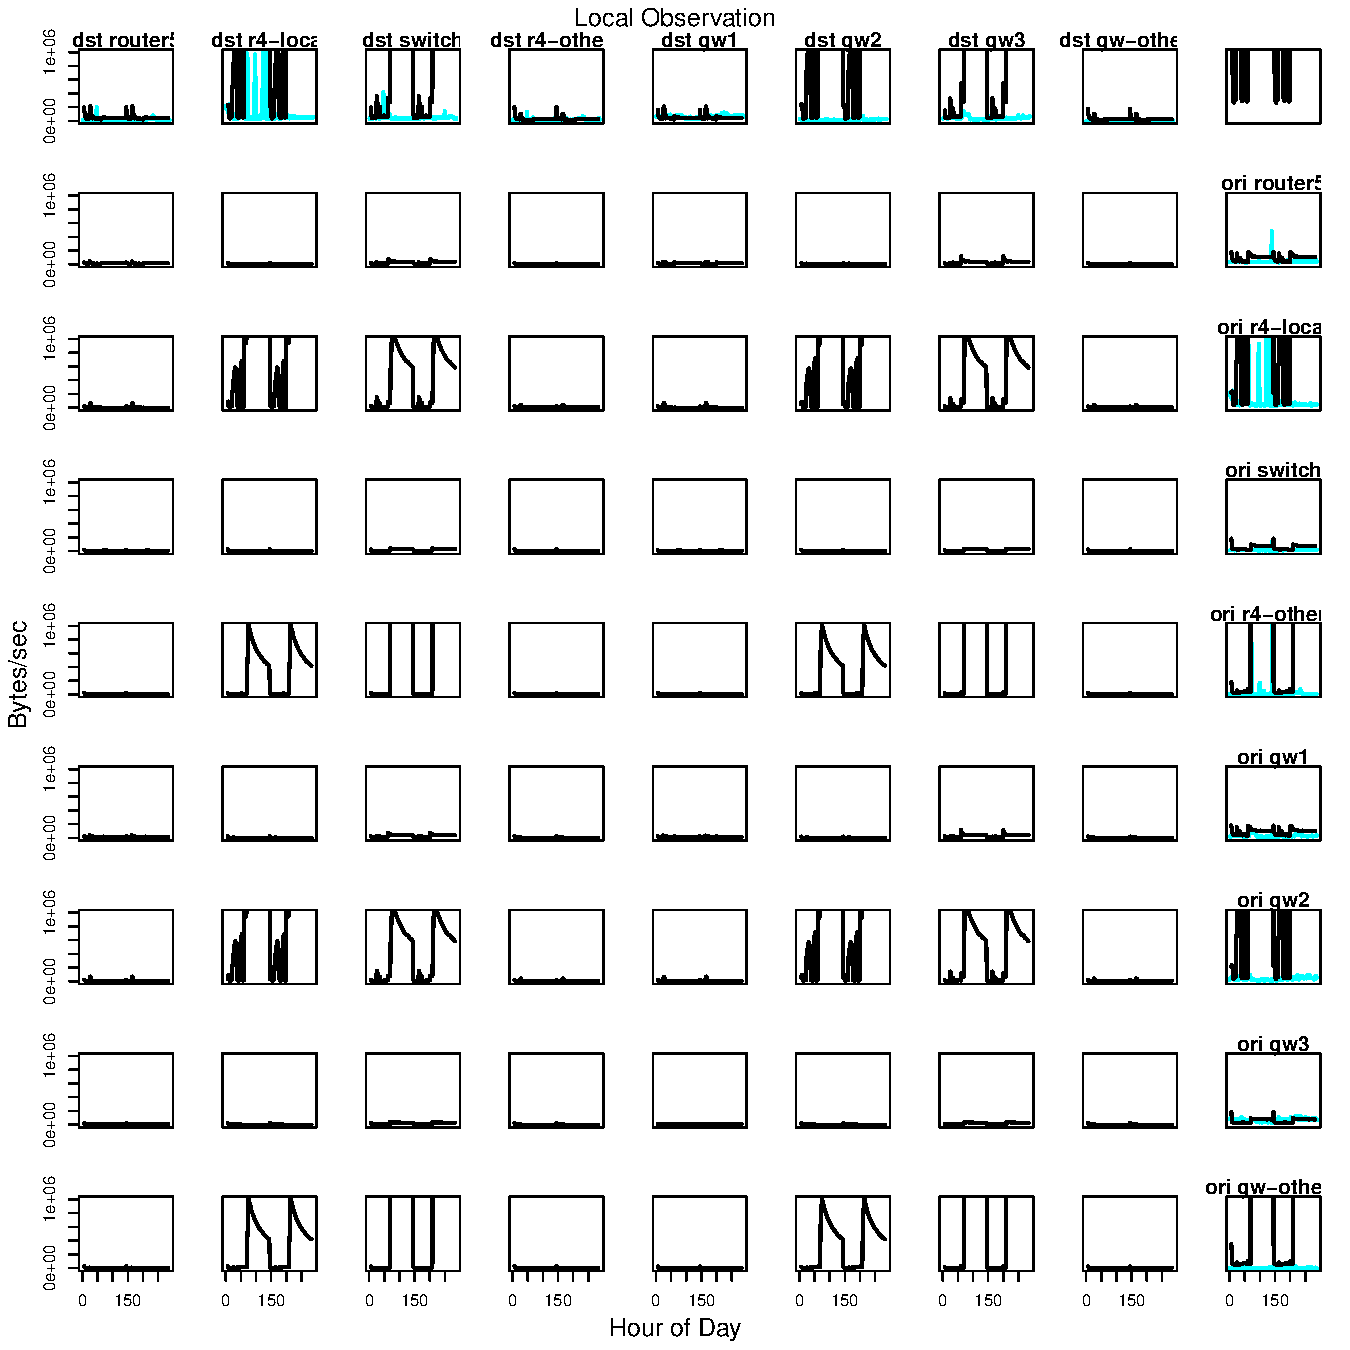
\includegraphics[scale=0.7]{tam_gregory_fig6_2routerlocal.pdf}
\end{center}
\begin{center}
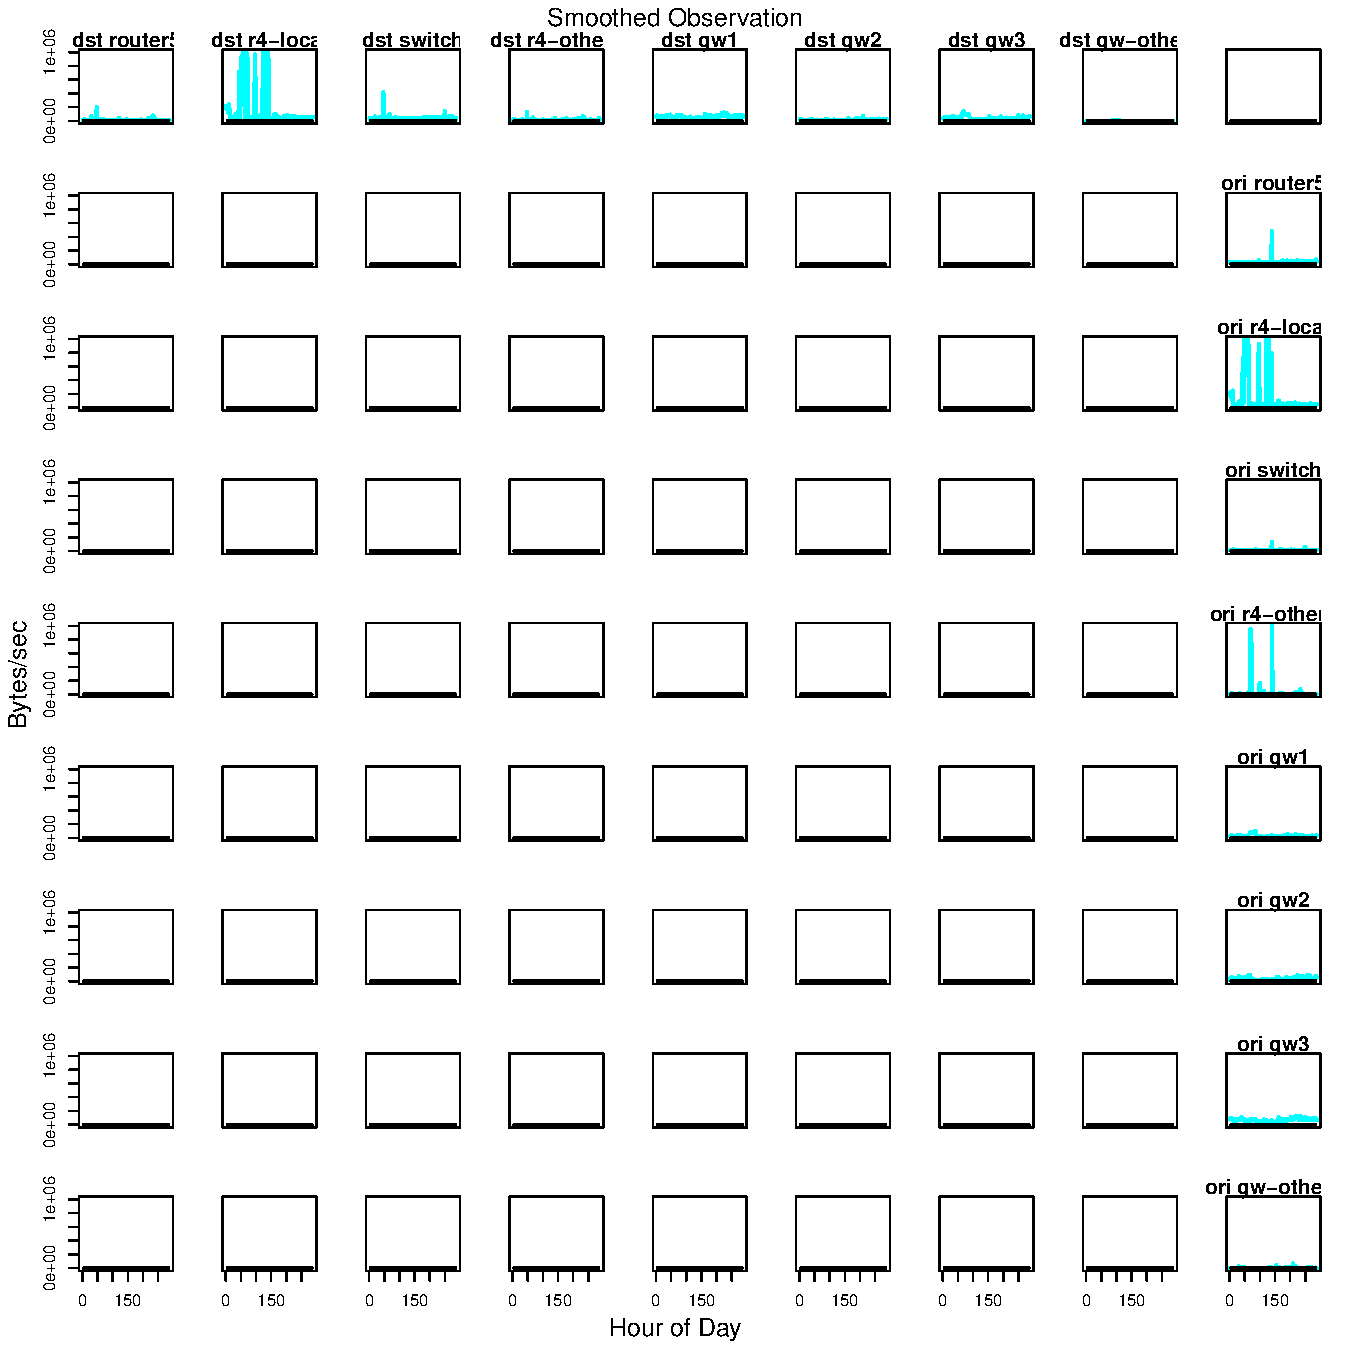
\includegraphics[scale=0.7]{tam_gregory_fig6_2router.pdf}
\end{center}


\item


\end{enumerate}
\end{document}

